% Template file for a standard thesis
\documentclass[11pt,notitlepage]{isuthesis}
% notitlepage is used because \begin{abstract} uses titlepage by default, which resets the page numbers

\usepackage[pdftex]{graphicx}
% Standard, old-style thesis
\usepackage{isutraditional}
\chaptertitle
% Old-style, thesis numbering down to subsubsection
\alternate
\usepackage{rotating}

% Bibliography
\usepackage{natbib}
\usepackage{chapterbib}
\bibliographystyle{plain}  % changed from apa, abbrv, unsrtnat

%\renewcommand\bibsection{\section*{\ref name}}
%\renewcommand\bibsection{\section*}
% \renewcommand{\bibsection}{\section{References}}


%\includeonly{titletoc,chapter1}
%Optional Package to add PDF bookmarks and hypertext links
\usepackage[pdftex,hypertexnames=false,linktocpage=true]{hyperref}
\hypersetup{colorlinks=true,linkcolor=blue,anchorcolor=blue,citecolor=blue,filecolor=blue,urlcolor=blue,bookmarksnumbered=true,pdfview=FitB}

%\usepackage{titletoc}

\overfullrule=0pt
%%%%%%%%%%%%%%%%%%%%%

% The following piece of code removes extra space on the top of each chapter
%  that is default of latex report class documents

\usepackage{etoolbox}
\makeatletter
\patchcmd{\@makechapterhead}{50\p@}{0pt}{}{}
\patchcmd{\@makeschapterhead}{50\p@}{0pt}{}{}
\makeatother

%%%%%%%%%%%%%%%%%%%%%%%
%%%%%%%%%%%%%%%%%%%%%%%%%
% Removing Bold characters in the Table of Contents
% % Alternatively to this the isuthesis.cls file has been changed by default in the
% % line section \renewcommand{\l@chapter}[2]{\addpenalty{-\@highpenalty}....
%\titlecontents{chapter}
%[0pt]                                               % left margin
%{}%
%{\contentsmargin{0pt}                               % numbered entry format
%    \thecontentslabel\enspace%
%    \large}
%{\contentsmargin{0pt}\large}                        % unnumbered entry format
%{\titlerule*[.5pc]{.}\contentspage}                 % filler-page format (e.g dots)
%[]                                                  % below code (e.g vertical space)
%%%%%%%%%%%%%%%%%%%%%%%%%%

%%%%%%%%%%%%%%%%%%%%%%%%%%%%%%%
% In order to change space between the Table of contents items go to isuthesis.cls
% line  \renewcommand{\l@chapter}[2]{\addpenalty{-\@highpenalty}....
% change \vkip values

%%%%%%%%%%%%%%%%%%%%%%%%%%
%% This is to minimize orphan lines. Might not be possible to entirely remove them
% Method 1 of doing this
\widowpenalty100000
\clubpenalty100000

% Method 2 of doing this
\usepackage[all]{nowidow}
%%%%%%%%%%%%%%%%%%%%%%%%%%%

%%% control bibliography spacings
% \newlength{\bibitemsep}\setlength{\bibitemsep}{\baselineskip}
% % plus .05\baselineskip minus .05\baselineskip}
% \newlength{\bibparskip}\setlength{\bibparskip}{0pt}
% \let\oldthebibliography\thebibliography
% \renewcommand\thebibliography[1]{%
%   \oldthebibliography{#1}%
%   \setlength{\parskip}{\bibitemsep}%
%   \setlength{\itemsep}{\bibparskip}%
% }
% \usepackage{setspace}
% \setlength{\bibsep}{2sp}


%%%%%%%%%%%%%%%%%%%%%%%%%%%%%%%%%%
% %% aligning lof captions
% \usepackage{tocloft}

%%%%%%%%%%%%%%%%%%%%%%%%%%%%%%%%%%
%% Set the margins in the whole document
\geometry{letterpaper, left=1in, top=1in, right=1in, bottom=1in, includehead=true}
%%%%%%%%%%%%%%%%%%%%%%%%%%%%%%%%%%

\usepackage{Logemann}
\usepackage{Sum}
\usepackage{Derivative}
\usepackage{Integral}
\renewcommand{\v}[1]{\mathbf{#1}}

\begin{document}

\DeclareGraphicsExtensions{.jpg,.pdf,.mps,.png}
%\begin{singlespace}
\def\@makechapterheada{\vspace*{-2cm}\titlepage} % in order to reduce the space between margin and heading in titlepage
% Template Titlepage File
% Please choose appropriate options for Master's thesis, Doctoral dissertations, and creative components. Please read the comments to make an informed choice

\@makechapterheada\titlepage  % using definition from thesis.tex reduce the space between margin and heading in titlepage
\title{Nonconservative discontinuous Galerkin methods for shallow water moment models}

\author{Caleb Logemann}

%%%%%%%%%%%%%%%%%%%
%% Master of Science options.
%% CC will have a couple of changes mentioned near the end of this file.

\degree{DOCTOR OF PHILOSOPHY}
\major{Applied Mathematics}

\level{master's}
\mprof{James Rossmanith}

\format{dissertation}
\committee{4}
\members{Hailiang Liu \\ Songting Luo \\ Alric Rothmayer \\ Jue Yan \\}
\disclaimertitlepage{The student author, whose presentation of the scholarship
    herein was approved by the program of study committee, is solely responsible
    for the content of this dissertation/thesis.
    The Graduate College will ensure this dissertation/thesis is globally
    accessible and will not permit alterations after a degree is conferred.}
%{The student author and the program of study committee are solely responsible for the content of this dissertation/thesis. The Graduate College will ensure this dissertation/thesis is globally accessible and will not permit alterations after a degree is conferred.}


%%%%%%%%%%%%%%%%%%%%%%%%%%%%
% Doctor of Philosophy options
% If co-majors select only co-major options as described and skip other options like \major, \mprof and make sure committee members are appropriately included.


% Add these additional lines for a Doctoral Dissertation
%\degree{DOCTOR OF PHILOSOPHY}
% \major{Human Development and Family Studies (Marriage and Family Therapy)}
% Use the following line for co-majors (usually used with doctoral dissertations)
%\comajors{Statistics; Computer Science}{}
%\level{doctoral}
%\mprof{Susan D. Ross}

%\format{dissertation}
%\committee{4}
%\members{Mary Jones \\ Bjork Petersen \\ Sam Anders \\ Harold Jones}
%\disclaimertitlepage{The student author, whose presentation of the scholarship herein was approved by the program of study committee, is solely responsible for the content of this dissertation/thesis. The Graduate College will ensure this dissertation/thesis is globally accessible and will not permit alterations after a degree is conferred.}

\notice
\maketitle

%\end{singlespace}
% Optional thesis dedication
% \chapter*{DEDICATION}

I would like to dedicate this thesis to my wife Glenda and
to my daughter Alice without whose support I would not have
been able to complete this work.


% Table of Contents, List of Tables and List of Figures
{
\pdfbookmark[1]{TABLE OF CONTENTS}{table}
\tableofcontents
}
%%%%%%%%%%%%%%%%%%%%%%%%%%%%%%%%%%%%%%%%%
%% The line below adds the word "Page" over the page numbers in TOC, LOT, LOF
\addtocontents{toc}{~\hfill\textbf{Page}\par}
\addtocontents{lot}{~\hfill\textbf{Page}\par}
\addtocontents{lof}{~\hfill\textbf{Page}\par}
%%
\addtocontents{toc}{\def\protect \@chapapp{}} \cleardoublepage \phantomsection
\pagebreak
\addcontentsline{toc}{chapter}{LIST OF TABLES}
%%%%%%%%%%%%%%%%%%%%%%%%%%%%%%%%%%%%%%%%%
\listoftables
\cleardoublepage \phantomsection \addcontentsline{toc}{chapter}{LIST OF FIGURES}
%%%%%%%%%%%%%%%%%%%%%%%%%%%%%%%%%%%%%%%%%
\listoffigures


% Comment out the next line if NOT using chaptertitle
\addtocontents{toc}{\def\protect\@chapapp{CHAPTER\ }}
%Optional Acknowledgements
\cleardoublepage \phantomsection
% \specialchapt{ACKNOWLEDGMENTS}

I would like to take this opportunity to express my thanks to those
who helped me with various aspects of conducting research and the writing
of this thesis.
First and foremost, Dr. Susan D. Ross for her guidance, patience and support
throughout this research and the writing of this thesis.
Her insights and words of encouragement have often inspired me and renewed
my hopes for completing my graduate education.
I would also like to thank my committee members for their efforts
and contributions to this work: Dr. August Tanner and
Dr. Lewis Hargrave.
I would additionally like to thank
Dr. Tanner for his guidance throughout the initial stages of my
graduate career and Dr. Hargrave for his inspirational teaching style.

%Optional thesis abstract
\cleardoublepage \phantomsection
\specialchapt{ABSTRACT}

I present a discontinuous Galerkin method for the generalized shallow water equations
first introduced by Kowalski and Torrilhon.
These generalized shallow water equations introduce vertical moments into the shallow
flow's velocity profile.
As a result of these additional moments a nonconservative term appears in these
hyperbolic equations.
We use the Dal Maso, Le Floch, and Murat theory of nonlinear hyperbolic systems in
nonconservative form to correctly discretize this nonconservative term.
Using this theory a high order discontinuous Galerkin method is presented for the
generalized equations in two dimensions

\newpage
\pagenumbering{arabic}

% Chapter 1 of the Thesis Template File
\chapter{Introduction}

In this paper we look at the model equation,
\begin{equation}
  q_t + \p{q^2 - q^3}_x = -\p{q^3 q_{xxx}}_x \quad (x, t) \in \br{a, b} \times \br{0, T}. \label{eq:thin_film_model}
\end{equation}
This equation describes the motion of a thin film of liquid flowing over a one-dimensional domain,
where \(q(x, t) \ge 0\) is the height of the liquid.
This fluid is acted upon by gravity, by forces on the surface, and by surface tension.
An equivalent model can be derived using thermocapillary forces and molecular forces.
This model is useful in many different applications including airplane de-icing\cite{}
and industrial coating.
Some experimental study~\cite{article:cazabat1990fingering,
article:kataoka1997theoretical, article:ludviksson1971dynamics} has been done and
numerical results have shown good agreement with those experiments
in~\cite{article:bertozzi1998contact}.

Previous numerical methods for this type of equation have focused on finite difference
approaches.
Bertozzi and Brenner\cite{bertozzi1997linear} used a fully implicit centered finite
difference scheme to explore instabilities.
Ha et al.\cite{article:Ha2008} explored several different finite difference schemes,
some fully implicit and some using the Crank-Nicolson method.
In their analysis the considered several different methods for the hyperbolic terms
including WENO, Godunov, and an adapted Upwind method.
All of these methods were limited to just first or second order, and they required
solving a Newton iteration.
Finite difference methods also lack provable stability.
% other drawbacks to finite difference methods

We chose to use discontinuous Galerkin methods as they allow for high order
convergence.
The discontinuous Galerkin methods were first introduced by Reed and
Hill\cite{techreport:Reed1973}, and then were formalized by Cockburn and Shu
in a series of papers\cite{article:Cockburn1991I, article:Cockburn1989II,
article:Cockburn1989III, article:Cockburn1990IV, article:cockburn1998V}.
We use the original modal discontinuous Galerkin method as well as the local
discontinuous Galerkin method.
The local discontinuous Galerkin method was also formulated by Cockburn and
Shu\cite{article:Cockburn1998LDG} to handle higher order derivatives with the
discontinuous Galerkin method.
We use the modal discontinuous Galerkin method to discretize the convection term and
the local discontinuous Galerkin method to discretize the diffusion term.

The diffusion term is much stiffer of a problem then the hyperbolic convection.
If the diffusion is handled explicitly in time, then a very strict time step
restriction is present for stability.
Therefore implicit schemes should be preferred.
However the hyperbolic term is nonlinear, and so an implicit scheme would require a
Newton iteration.
Thus we chose to use an Implicit-Explicit Runge Kutta scheme for propagating in time.
These schemes were first introduced by Ascher et al.\cite{article:ascher1997implicit}
and have been expanded on by Kennedy and Carpenter\cite{kennedy2003additive} and
Pareschi and Russo\cite{article:pareschi2000IMEX}.
\clearpage
\pagebreak

% !TEX root = ../../thesis.tex

\chapter{The Thin-Film Model}
  In this model we consider a thin film of liquid on a flat surface with a free interface.
  This liquid is driven by gravity, shear and normal forces on the surface, and surface
  tension (see Figure~\ref{fig:thin_film}).
  We begin by considering the two dimensional incompressible Navier-Stokes equations,
  which have the form,
  \begin{align}
    u_x + w_z &= 0, \label{eq:incompressibility}\\
    \rho\p{u_t + u u_x + w u_z} &= -p_x + \mu \Delta u - \phi_x, \label{eq:con_mom1}\\
    \rho\p{w_t + u w_x + w w_z} &= -p_z + \mu \Delta w - \phi_z, \label{eq:con_mom2}
  \end{align}
  where \(\rho \) is the density, \(u\) is the horizontal velocity, \(w\) is the
  vertical velocity, \(p\) is the pressure, and \(\phi \) is the force of gravity.
  Equation~\eqref{eq:incompressibility} is the incompressibility condition and also
  represents conservation of mass.
  Equations~\eqref{eq:con_mom1} and~\eqref{eq:con_mom2} represent the conservation of
  momentum in the \(x\) and \(z\) directions respectively.
  We take a no penetration and no slip boundary condition at the lower boundary and the
  kinematic boundary condition at the upper boundary.
  These boundary conditions can be expressed as follows,
  \begin{align}
    w &= 0, u = 0, &\text{at } z = 0, \\
    w &= h_t + u h_x, &\text{at } z = h,
  \end{align}
  where \(h\) is the height of the liquid.
  We can also describe the stress tensor, \(\v{T}\), at the free surface, \(z = h\),
  as
  \begin{align*}
    \v{T} \cdot \v{n} &= \p{-\kappa \sigma + \Pi_0}\v{n}
      + \p{\pd{\sigma}{s} + \tau_0}\v{t}, &\text{at } z = h,
  \end{align*}
  where \(\kappa \) is the mean curvature, \(\sigma \) is the surface tension, and
  \(\Pi_0 \) and \(\tau_0 \) are the normal and tangential components of the forcing
  respectively.

  \begin{figure}[ht]
    \centering
    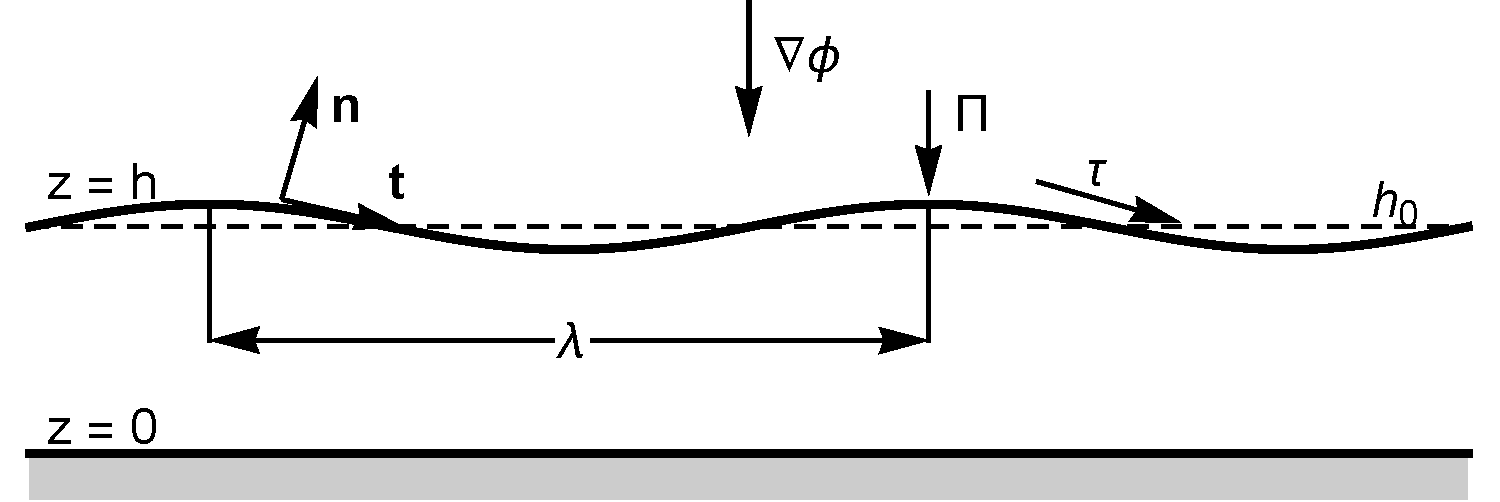
\includegraphics[scale=0.45]{figures/ThinFilm.pdf}
    \caption{A diagram of the Thin-Film Model}\label{fig:thin_film}
  \end{figure}

\subsection{Derivation}
  These equations completely describe the fluid, but we are now going to make a
  lubrication approximation, through a scaling argument similar to that given by Oron
  et al.~\cite{oron1997long}.
  For the lubrication approximation we are going to assume that the average height of
  the liquid, \(h_0\), is much smaller then the characteristic wavelength of the liquid,
  \(\lambda \).
  We will denote the ratio of these two lengths as \(\varepsilon \), that is
  \begin{equation}
    \varepsilon = \frac{h_0}{\lambda} \ll 1.
  \end{equation}
  Now we nondimensionalize the rest of the variables with respect to this ratio.
  We denote the nondimensional variables as the uppercase variables.
  As we stated earlier the characteristic height is \(h_0\) and the characteristic
  length is \(\lambda = h_0/\varepsilon \), so the nondimensional length variables are
  \begin{equation}
    Z = \frac{z}{h_0}, \quad X = \frac{\varepsilon x}{h_0}, \quad H = \frac{h}{h_0}.
  \end{equation}
  Let \(U_0\) be the characteristic horizontal velocity, then
  \begin{equation}
    \quad U = \frac{u}{U_0}, \quad W = \frac{w}{\varepsilon U_0},
  \end{equation}
  where the nondimensional vertical velocity, \(W\), follows from the continuity
  equation, equation~\eqref{eq:incompressibility}.
  It follows that time will be scaled by \(\lambda/U_0\), so nondimensional time is
  \begin{equation}
    T = \frac{\varepsilon U_0 t}{h_0}.
  \end{equation}
  Finally we assume that the flow is locally parallel or equivalently
  \(p_x \sim \mu u_{zz}\).
  This gives us the proper scaling for the pressure, gravity, and surface stresses,
  \begin{equation}
    P = \frac{\varepsilon h_0}{\mu U_0} p, \quad
    \Phi = \frac{\varepsilon h_0}{\mu U_0}\phi, \quad
    \Pi = \frac{\varepsilon h_0}{\mu U_0}\Pi_0, \quad
    \tau = \frac{h_0}{\mu U_0}\tau_0.
  \end{equation}
  Lastly we can nondimensionalize the surface tension as
  \begin{equation}
    \Sigma = \frac{\varepsilon \sigma}{\mu U_0}.
  \end{equation}

%   The following give some intermediate steps in how to nondimensionalize variables
%   that include derivatives.
%   \begin{align*}
%     u_x &= U_0 U_X \pd{X}{x} = \frac{\varepsilon U_0}{h_0} U_X\\
%     w_z &= \varepsilon U_0 W_Z \pd{Z}{z} = \frac{\varepsilon U_0}{h_0} W_Z \\
%     u_t &= U_0 U_T \pd{T}{t} = \frac{\varepsilon U_0^2}{h_0} U_T \\
%     uu_x &= U_0 U U_0 U_X \pd{X}{x} = \frac{\varepsilon U_0^2}{h_0} UU_X \\
%     wu_z &= \varepsilon U_0 W U_0 U_Z \pd{Z}{z} = \frac{\varepsilon U_0^2}{h_0} WU_Z \\
%     w_t &= \varepsilon U_0 W_T \pd{T}{t} = \frac{\varepsilon^2 U_0^2}{h_0} W_T \\
%     uw_x &= U_0 U \varepsilon U_0 W_X \pd{X}{x} = \frac{\varepsilon^2 U_0^2}{h_0} UW_X \\
%     ww_z &= \varepsilon U_0 W \varepsilon U_0 W_Z \pd{Z}{z} = \frac{\varepsilon^2 U_0^2}{h_0} WW_Z \\
%     p_x &= \frac{\mu U_0}{\varepsilon h_0} P_X \pd{X}{x} = \frac{\mu U_0}{h_0^2} P_X \\
%     p_z &= \frac{\mu U_0}{\varepsilon h_0} P_Z \pd{Z}{z} = \frac{\mu U_0}{\varepsilon h_0^2} P_Z \\
%     u_{xx} &= U_0 U_{XX} \p{\pd{X}{x}}^2 = \frac{\varepsilon^2 U_0}{h_0^2} U_{XX} \\
%     u_{zz} &= U_0 U_{ZZ} \p{\pd{Z}{z}}^2 = \frac{U_0}{h_0^2} U_{ZZ} \\
%     w_{xx} &= \varepsilon U_0 W_{XX} \p{\pd{X}{x}}^2 = \frac{\varepsilon^3 U_0}{h_0^2} W_{XX} \\
%     w_{zz} &= \varepsilon U_0 U_{ZZ} \p{\pd{Z}{z}}^2 = \frac{\varepsilon U_0}{h_0^2} W_{ZZ} \\
%     \phi_x &= \frac{\mu U_0}{\varepsilon h_0} \Phi_X \pd{X}{x} = \frac{\mu U_0}{h_0^2} \Phi_X \\
%     \phi_z &= \frac{\mu U_0}{\varepsilon h_0} \Phi_Z \pd{Z}{z} = \frac{\mu U_0}{\varepsilon h_0^2} \Phi_Z \\
%     h_t &= h_0 H_T \pd{T}{t} = \varepsilon U_0 H_T \\
%     u h_x &= U_0 U h_0 H_X \pd{X}{x} = \varepsilon U_0 U H_X
%   \end{align*}

  Substituting these nondimensional variables into the continuity
  equation~\eqref{eq:incompressibility}, gives
  \begin{align*}
    u_x + w_z &= 0, \\
    \frac{\varepsilon U_0}{h_0} U_X + \frac{\varepsilon U_0}{h_0} W_Z &= 0, \\
    U_X + W_Z &= 0.
  \end{align*}
  This computation also justifies the scaling of \(w\) as the nondimensional variables
  should also conserve mass.

  We can nondimensionalize the conservation of momentum equations as follows,
  \begin{align*}
    \rho\p{u_t + u u_x + w u_z} &= -p_x + \mu \Delta u - \phi_x, \\
    \rho\p{\frac{\varepsilon U_0^2}{h_0} U_T + \frac{\varepsilon U_0^2}{h_0} UU_X
    + \frac{\varepsilon U_0^2}{h_0} WU_Z} &= -\frac{\mu U_0}{h_0^2} P_X
    + \mu \p{\frac{\varepsilon^2 U_0}{h_0^2} U_{XX} + \frac{U_0}{h_0^2} U_{ZZ}}
    - \frac{\mu U_0}{h_0^2} \Phi_X, \\
    \frac{\varepsilon U_0^2 \rho}{h_0}\p{U_T + UU_X + WU_Z} &=
    \frac{\mu U_0}{h_0^2}\p{-P_X + \p{\varepsilon^2 U_{XX} + U_{ZZ}} - \Phi_X }, \\
    \frac{\varepsilon U_0 \rho h_0}{\mu}\p{U_T + UU_X + WU_Z} &=
    \p{-P_X + \p{\varepsilon^2 U_{XX} + U_{ZZ}} - \Phi_X },
  \end{align*}
  and
  \begin{align*}
    \rho\p{w_t + u w_x + w w_z} &= -p_z + \mu \Delta w - \phi_z, \\
    \rho\p{\frac{\varepsilon^2 U_0^2}{h_0} W_T + \frac{\varepsilon^2 U_0^2}{h_0} UW_X
    + \frac{\varepsilon^2 U_0^2}{h_0} WW_Z} &= -\frac{\mu U_0}{\varepsilon h_0^2} P_Z
    + \mu \p{\frac{\varepsilon^3 U_0}{h_0^2} W_{XX}
    + \frac{\varepsilon U_0}{h_0^2} W_{ZZ}}
    - \frac{\mu U_0}{\varepsilon h_0^2} \Phi_Z, \\
    \frac{\varepsilon^2 \rho U_0^2}{h_0}\p{W_T + UW_X + WW_Z} &=
    \frac{\mu U_0}{\varepsilon h_0^2} \p{-P_Z
    + \p{\varepsilon^4 W_{XX} + \varepsilon^2 W_{ZZ}} - \Phi_Z}, \\
    \varepsilon^3 \frac{\rho U_0 h_0}{\mu}\p{W_T + UW_X + WW_Z} &=
    \p{-P_Z + \varepsilon^2\p{\varepsilon^2 W_{XX} + W_{ZZ}} - \Phi_Z}.
  \end{align*}

  The boundary conditions are nondimensionalized as below,
  \begin{align*}
    w &= 0, \quad u = 0, &\text{at } z = 0, \\
    \varepsilon U_0 W &= 0, \quad U_0 U = 0, &\text{at } Z = 0, \\
    W &= 0, \quad U = 0, &\text{at } Z = 0,
  \end{align*}
  with
  \begin{align*}
    w &= h_t + u h_x, &\text{at } z = h, \\
    \varepsilon U_0 W &= \varepsilon U_0 H_T + \varepsilon U_0 U H_x, &\text{at } Z = H, \\
    W &= H_T + U H_x, &\text{at } Z = H.
  \end{align*}

  In order to nondimensionalize the stress tensor at the free surface, we consider the
  normal and tangential components of \(\v{T} \cdot \v{n}\) separately.
  The normal and tangential vector at the surface can be expressed in terms of the free
  surface as
  \begin{gather}
    \v{n} = \frac{\abr{-h_x, 1}}{\p{1 + h_x^2}^{1/2}}, \quad
    \v{t} = \frac{\abr{1, h_x}}{\p{1 + h_x^2}^{1/2}},
  \end{gather}
  and the mean curvature, \(\kappa \), can be expressed in terms of \(h\) as
  \begin{equation}
    \kappa = -\frac{h_{xx}}{\p{1 + h_x^2}^{3/2}}.
  \end{equation}
  We would now like to write the following vector equation in terms of its normal and
  tangential components.
  \begin{align*}
    \v{T} \cdot \v{n} &= \p{-\kappa \sigma + \Pi_0}\v{n}
      + \p{\pd{\sigma}{s} + \tau_0}\v{t}, &\text{at } z = h.
  \end{align*}

  Note that we are using a Newtonian stress tensor which is given by
  \begin{align}
    \v{T} &=
    \begin{bmatrix}
      -p & 0 \\
      0 & -p
    \end{bmatrix} +
    \mu \begin{bmatrix}
      2u_x & u_z + w_x \\
      u_z + w_x & 2w_z
    \end{bmatrix}
  \end{align}

  The normal component of this vector equation is given by
  \begin{align}
    \abr{\v{T} \cdot \v{n}, \v{n}} &= \p{-\kappa \sigma + \Pi_0}.
  \end{align}

  First we will simplify the left hand side.
  \begin{align*}
    a &= \p{1 + h_x^2}^{1/2}, \\
    \abr{\v{T} \cdot \v{n}, \v{n}} &= \frac{1}{a^2}
    \begin{bmatrix}
      -h_x & 1
    \end{bmatrix}
    \begin{bmatrix}
      -p + 2 \mu u_x & \mu \p{u_z + w_x} \\
      \mu \p{u_z + w_x} & -p + 2 \mu w_z
    \end{bmatrix}
    \begin{bmatrix}
      -h_x \\
      1
    \end{bmatrix}, \\
    &=
    \frac{1}{a^2}
    \begin{bmatrix}
      -h_x & 1
    \end{bmatrix}
    \begin{bmatrix}
      -h_x \p{-p + 2 \mu u_x} + \mu \p{u_z + w_x} \\
      -h_x \mu \p{u_z + w_x} + -p + 2\mu w_z
    \end{bmatrix}, \\
    &= \frac{1}{a^2} \p{h_x^2\p{-p + 2\mu u_x} - \mu h_x \p{u_z + w_x}
      - \mu h_x \p{u_z + w_x} + -p + 2\mu w_z}, \\
    &= \frac{1}{a^2} \p{h_x^2\p{-p + 2 \mu u_x}
      - 2 \mu h_x \p{u_z + w_x} - p + 2\mu w_z}, \\
    &= \frac{1}{a^2} \p{\p{1 + h_x^2} \p{-p} + 2 \mu \p{h_x^2 u_x + w_z}
      - 2 \mu h_x \p{u_z + w_x}}, \\
    &= -p + \frac{2 \mu}{a^2} \p{\p{h_x^2 u_x + w_z}
      - h_x \p{u_z + w_x}}.
  \end{align*}
  Next simplify the right hand side,
  \begin{align*}
    \p{-\kappa \sigma + \Pi_0} &= \frac{h_{xx}}{\p{1 + h_x^2}^{3/2}} \sigma + \Pi_0.
  \end{align*}
  This gives the following scalar equation,
  \begin{align}
    -p - \Pi_0 + \frac{2 \mu}{1 + h_x^2} \p{\p{h_x^2 u_x + w_z}
      - h_x \p{u_z + w_x}} &= \frac{h_{xx}}{\p{1 + h_x^2}^{3/2}} \sigma.
  \end{align}

  The tangential component is given by
  \begin{align}
    \abr{\v{T} \cdot \v{n}, \v{t}} &= \p{\pd{\sigma}{s} + \tau_0}.
  \end{align}
  First simplify the left hand side,
  \begin{align*}
    \abr{\v{T} \cdot \v{n}, \v{n}} &= \frac{1}{a^2}
    \begin{bmatrix}
      1 & h_x
    \end{bmatrix}
    \begin{bmatrix}
      -p + 2 \mu u_x & \mu \p{u_z + w_x} \\
      \mu \p{u_z + w_x} & -p + 2 \mu w_z
    \end{bmatrix}
    \begin{bmatrix}
      -h_x \\
      1
    \end{bmatrix}, \\
    &=
    \frac{1}{a^2}
    \begin{bmatrix}
      1 & h_x
    \end{bmatrix}
    \begin{bmatrix}
      -h_x \p{-p + 2 \mu u_x} + \mu \p{u_z + w_x} \\
      -h_x \mu \p{u_z + w_x} + -p + 2\mu w_z
    \end{bmatrix}, \\
    &= \frac{1}{a^2} \p{-h_x \p{-p + 2 \mu u_x} + \mu \p{u_z + w_x}
      + -h_x^2 \mu \p{u_z + w_x} + h_x \p{-p + 2\mu w_z}}, \\
    &= \frac{1}{a^2} \p{-h_x \p{2 \mu u_x} + \mu \p{u_z + w_x}
      + -h_x^2 \mu \p{u_z + w_x} + h_x \p{2\mu w_z}}, \\
    &= \frac{\mu}{a^2} \p{2 h_x \p{w_z - u_x} + \p{1 - h_x^2} \p{u_z + w_x}}.
  \end{align*}
  Next simplify the right hand side
  \begin{align*}
    \p{\pd{\sigma}{s} + \tau_0} &= \pd{\sigma}{x} \pd{x}{s} + \tau_0, \\
    &= \pd{\sigma}{x} \frac{1}{\p{1 + h_x^2}^{1/2}} + \tau_0.
  \end{align*}
  This gives the following scalar equation,
  \begin{align}
    \mu \p{2 h_x \p{w_z - u_x} + \p{1 - h_x^2} \p{u_z + w_x}} &= \pd{\sigma}{x} \p{1 + h_x^2}^{1/2} + \tau_0\p{1 + h_x^2}.
  \end{align}

  Lastly we will nondimensionalize these two equations,
  \begin{gather*}
    -p - \pi + \frac{2 \mu}{1 + h_x^2} \p{\p{h_x^2 u_x + w_z}
      - h_x \p{u_z + w_x}} = \frac{h_{xx}}{\p{1 + h_x^2}^{3/2}} \sigma, \\
    -\frac{\mu U_0}{\varepsilon h_0}P - \frac{\mu U_0}{\varepsilon h_0}\Pi + \frac{2 \mu}{1 + \varepsilon^2 H_X^2} \p{\p{\varepsilon^2 H_X^2 \frac{\varepsilon U_0}{h_0} U_X + \frac{\varepsilon U_0}{h_0} W_Z}
      - \varepsilon H_X \p{\frac{U_0}{h_0} U_Z + \frac{\varepsilon^2 U_0}{h_0} W_X}} \\
      = \frac{\varepsilon^2}{h_0}\frac{H_{XX}}{\p{1 + \varepsilon^2 H_X^2}^{3/2}} \frac{\mu U_0}{\varepsilon} \Sigma, \\
    \p{-\frac{\mu U_0}{\varepsilon h_0}P - \frac{\mu U_0}{\varepsilon h_0}\Pi + \frac{\varepsilon \mu U_0}{h_0}\frac{2}{1 + \varepsilon^2 H_X^2} \p{\p{\varepsilon^2 H_X^2 U_X + W_Z}
      - H_X \p{U_Z + \varepsilon^2 W_X}}} \\
      = \frac{\varepsilon \mu U_0}{h_0}\frac{H_{XX}}{\p{1 + \varepsilon^2 H_X^2}^{3/2}} \Sigma, \\
    \p{-\frac{\mu U_0}{\varepsilon h_0}P - \frac{\mu U_0}{\varepsilon h_0}\Pi + \frac{\varepsilon \mu U_0}{h_0}\frac{2}{1 + \varepsilon^2 H_X^2} \p{\p{\varepsilon^2 H_X^2 U_X + W_Z}
      - H_X \p{U_Z + \varepsilon^2 W_X}}} \\
      = \frac{\varepsilon \mu U_0}{h_0}\frac{H_{XX}}{\p{1 + \varepsilon^2 H_X^2}^{3/2}} \Sigma, \\
    \frac{\mu U_0}{\varepsilon h_0}\p{-P - \Pi + \frac{2 \varepsilon^2}{1 + \varepsilon^2 H_X^2} \p{\p{\varepsilon^2 H_X^2 U_X + W_Z}
      - H_X \p{U_Z + \varepsilon^2 W_X}}}
      = \frac{\mu U_0}{\varepsilon h_0}\frac{\varepsilon^2 H_{XX}}{\p{1 + \varepsilon^2 H_X^2}^{3/2}} \Sigma, \\
    \p{-P - \Pi + \frac{2 \varepsilon^2}{1 + \varepsilon^2 H_X^2} \p{\p{\varepsilon^2 H_X^2 U_X + W_Z}
      - H_X \p{U_Z + \varepsilon^2 W_X}}}
      = \frac{\varepsilon^2 H_{XX}}{\p{1 + \varepsilon^2 H_X^2}^{3/2}} \Sigma,
  \end{gather*}
  and
  \begin{gather*}
    \mu \p{2 h_x \p{w_z - u_x} + \p{1 - h_x^2} \p{u_z + w_x}} = \pd{\sigma}{x} \p{1 + h_x^2}^{1/2} + \tau_0\p{1 + h_x^2}, \\
    \mu \p{2 \varepsilon H_X \p{\frac{\varepsilon U_0}{h_0} W_Z - \frac{\varepsilon U_0}{h_0} U_X}
    + \p{1 - \varepsilon^2 H_X^2} \p{\frac{U_0}{h_0} U_Z + \frac{\varepsilon^2 U_0}{h_0} W_X}} \\
    = \frac{\mu U_0}{h_0} \Sigma_X \p{1 + \varepsilon^2 H_X^2}^{1/2}
    + \frac{\mu U_0}{h_0} \tau \p{1 + \varepsilon^2 H_X^2}, \\
    \frac{\mu U_0}{h_0} \p{2 \varepsilon^2 H_X \p{W_Z - U_X}
    + \p{1 - \varepsilon^2 H_X^2} \p{U_Z + \varepsilon^2 W_X}} \\
    = \frac{\mu U_0}{h_0} \p{\Sigma_X \p{1 + \varepsilon^2 H_X^2}^{1/2}
    + \tau \p{1 + \varepsilon^2 H_X^2}}, \\
    2 \varepsilon^2 H_X \p{W_Z - U_X} + \p{1 - \varepsilon^2 H_X^2} \p{U_Z + \varepsilon^2 W_X} \\
    = \Sigma_X \p{1 + \varepsilon^2 H_X^2}^{1/2} + \tau \p{1 + \varepsilon^2 H_X^2}.
  \end{gather*}

  The full nondimensional equations are thus
  \begin{align}
    U_X + W_Z &= 0, \\
    \frac{\varepsilon U_0 \rho h_0}{\mu}\p{U_T + UU_X + WU_Z} &=
    -P_X + \p{\varepsilon^2 U_{XX} + U_{ZZ}} - \Phi_X, \\
    \varepsilon^3 \frac{\rho U_0 h_0}{\mu}\p{W_T + UW_X + WW_Z} &=
    -P_Z + \varepsilon^2\p{\varepsilon^2 W_{XX} + W_{ZZ}} - \Phi_Z,
  \end{align}
  at \(Z = 0\)
  \begin{gather}
    W = 0, \quad U = 0,
  \end{gather}
  and at \(Z = H\),
  \begin{gather}
    W = H_T + U H_x, \\
    -P - \Pi + \frac{2 \varepsilon^2}{1 + \varepsilon^2 H_X^2} \p{\p{\varepsilon^2 H_X^2 U_X + W_Z}
    - H_X \p{U_Z + \varepsilon^2 W_X}} = \frac{\varepsilon^2 H_{XX}}{\p{1 + \varepsilon^2 H_X^2}^{3/2}} \Sigma, \\
    2 \varepsilon^2 H_X \p{W_Z - U_X} + \p{1 - \varepsilon^2 H_X^2} \p{U_Z + \varepsilon^2 W_X}
    = \Sigma_X \p{1 + \varepsilon^2 H_X^2}^{1/2} + \tau \p{1 + \varepsilon^2 H_X^2}.
  \end{gather}

  We can now let \(\varepsilon \to 0\) which results in
  \begin{align}
    U_X + W_Z &= 0, \\
    P_X + \Phi_X &= U_{ZZ}, \\
    P_Z + \Phi_Z &= 0,
  \end{align}
  at \(Z = 0\),
  \begin{gather}
    W = 0, \quad U = 0, \\
  \end{gather}
  and at \(Z = H\)
  \begin{align}
    W &= H_T + U H_x, \\
    -P - \Pi &= \bar{\Sigma} H_{XX}, \\
    U_Z &= \Sigma_X + \tau.
  \end{align}
  Note that we assume that the surface tension is large, so that
  \(\bar{\Sigma} = \varepsilon^2 \Sigma = O(1)\).
  This is important in order to keep surface tension effects in the final equation.

  Next we integrate the continuity equation over \(Z\),
  \begin{align*}
    \dintt{0}{H}{U_X + W_Z}{Z} &= 0, \\
    \dintt{0}{H}{U_X}{Z} + \eval*{W}{Z = 0}{H} &= 0, \\
    \dintt{0}{H}{U_X}{Z} + H_T + U H_X &= 0, \\
    H_T + \dintt{0}{H}{U_X}{Z} + U H_X &= 0, \\
    H_T + \pda{\dintt{0}{H}{U}{Z}}{X} &= 0.
  \end{align*}

  Using the boundary conditions we can solve for an expression of \(U\) as follows
  \begin{align*}
    \dintt{Z}{H}{U_{ZZ}}{Z} &= \dintt{Z}{H}{P_X + \Phi_X}{Z}, \\
    \eval*{U_Z}{Z}{H} &= \p{P_X + \Phi_X}\p{H - Z}, \\
    \p{\tau + \Sigma_X} - U_Z &= \p{P_X + \Phi_X}\p{H - Z}, \\
    \dintt{0}{Z}{\p{\tau + \Sigma_X} - U_Z}{Z} &= \dintt{0}{Z}{\p{P_X + \Phi_X}\p{H - Z}}{Z}, \\
    \p{\tau + \Sigma_X}Z - \eval*{U}{Z = 0}{Z} &= \p{P_X + \Phi_X}\p{HZ - \frac{1}{2} Z^2}, \\
    \p{\tau + \Sigma_X}Z - U &= \p{P_X + \Phi_X}\p{HZ - \frac{1}{2} Z^2}, \\
    U &= \p{\tau + \Sigma_X}Z + \p{P_X + \Phi_X}\p{\frac{1}{2} Z^2 - HZ}.
  \end{align*}

  The boundary conditions also give an expression for \(P + \Phi \),
  \begin{align*}
    P_Z + \Phi_Z &= 0, \\
    \dintt{Z}{H}{P_Z + \Phi_Z}{Z} &= 0, \\
    \eval{P}{Z=H} - P + \eval{\Phi}{Z=H} - \Phi &= 0, \\
    -\Pi - \bar{\Sigma} H_{XX} - P + \eval{\Phi}{Z=H} - \Phi &= 0, \\
    P + \Phi &= \eval{\Phi}{Z=H} - \Pi - \bar{\Sigma} H_{XX}.
  \end{align*}

  Plugging both of these into the integrated continuity equation gives,
  \begin{align*}
    H_T + \pda{\dintt{0}{H}{U}{Z}}{X} &= 0, \\
    H_T + \pda{\dintt{0}{H}{\p{\tau + \Sigma_X}Z + \p{P_X + \Phi_X}\p{\frac{1}{2} Z^2 - HZ}}{Z}}{X} &= 0, \\
    H_T + \p{\frac{1}{2}\p{\tau + \Sigma_X}H^2 + \p{P_X + \Phi_X}\p{\frac{1}{6} H^3 - \frac{1}{2}H^3}}_X &= 0, \\
    H_T + \p{\frac{1}{2}\p{\tau + \Sigma_X}H^2 - \frac{1}{3}\p{P + \Phi}_X H^3}_X &= 0, \\
    H_T + \p{\frac{1}{2}\p{\tau + \Sigma_X}H^2 - \frac{1}{3}\p{\eval{\Phi}{Z=H} - \Pi - \bar{\Sigma} H_{XX}}_X H^3}_X &= 0, \\
    H_T + \p{\frac{1}{2}\p{\tau + \Sigma_X}H^2 - \frac{1}{3}\p{\eval{\Phi}{Z=H} - \Pi}_X H^3}_X &= - \p{\bar{\Sigma} H^3 H_{XXX}}_X.
  \end{align*}

  This is our final thin-film equation and taking all of the constants to be one gives
  \begin{equation}
    H_T + \p{H^2 - H^3}_X = - \p{H^3 H_{XXX}}_X.
  \end{equation}
  For the rest of the paper we will relabel the variables and use variables originally
  shown in equation~\ref{eq:thin_film_model},
  \begin{equation}
    q_t + \p{q^2 - q^3}_x = -\p{q^3 q_{xxx}}_x.
  \end{equation}

\subsection{Equation Properties}
  % TODO

% \bibliographystyle{plain}
% \begingroup
%     \setlength{\bibsep}{13.2pt}
%     \linespread{1}\selectfont
%     \bibliography{refs}
% \endgroup
\clearpage
\pagebreak
\chapter{PAPER 2 TITLE GOES HERE}
%\label{polymer_fibers}

\begin{center}
    A paper accepted by \textit{Name of the Journal} \\
    First Author and Second Author
\end{center}

\section{Abstract}
This is the text of my abstract that is part of the thesis itself.
The abstract describes the work in the first paper general. You can use the same abstract as your paper here.

%\pagebreak %remove if needed

% Please include sections as the paper has, some of the following sections are meant as examples of what can be done, the bibliography should be made as given

\section{Overview}

The  construct of this section or any further section is same as the authors paper.
This is the opening paragraph to my thesis which
explains in general terms the concepts and hypothesis
which will be used in my thesis.

With more general information given here than really
necessary.

\section{Introduction}

Here initial concepts and conditions are explained and
several hypothesis are mentioned in brief.

\cite{allen}, \cite{bruner} and \cite{cox}
did the initial work in this area. But in Struss' work [\cite{struss}]
the definitive model is seen.

\subsection{Hypothesis}

Here one particular hypothesis is explained in depth
and is examined in the light of current literature.

\subsubsection{Parts of the hypothesis}

Here one particular part of the hypothesis that is 
currently being explained is examined and particular
elements of that part are given careful scrutiny.

% Below \subsubsection
% Sectional commands: \paragraph and \subparagraph may also be used

\subsection{Second Hypothesis}

Here one particular hypothesis is explained in depth
and is examined in the light of current literature.

\subsubsection{Parts of the second hypothesis}

Here one particular part of the hypothesis that is 
currently being explained is examined and particular
elements of that part are given careful scrutiny.

\section{Criteria Review}

Here certain criteria are explained thus eventually
leading to a foregone conclusion.

\section{Conclusion}\label{Conclusion1}

The conclusion of the paper goes here.

\cite{allen}, \cite{bruner}, 
\cite{Hal82},
\cite{Rud73}, \cite{Con90}, 
\cite{Con78}, \cite{KR83}, 
\cite{KR86}

% This section may or may not be included
\section{Appendix: supplemental procedure description}
If there is an appendix that needs to go with the paper it can be as a section

\subsection{Procedure details}
Details of the paper specific appendix procedures

%\section{Bibliography}
\bibliographystyle{apa}
% \vspace{-20pt}
\begingroup
    \setlength{\bibsep}{13.2pt}
    \linespread{1}\selectfont
    \bibliography{master_bib}
\endgroup
\clearpage
\pagebreak
% !TEX root = ../../thesis.tex

\chapter{Results}\label{chp:results}
\section{Manufactured Solution}\label{ssec:manufactured_solution}
In order to confirm the order of accuracy of our method, we use the method of
manufactured solutions.
The method of manufactured solutions picks an exact solution \(\hat{q}\) and then adds
a source term to the initial partial differential equation to make \(\hat{q}\) the
true solution to the new differential equation.
So we actually solve
\begin{equation}
    q_t + \p{q^2 - q^3}_x = -\p{q^3 q_{xxx}}_x + s
\end{equation}
where
\begin{equation}
    s = \hat{q}_t + \p{\hat{q}^2 - \hat{q}^3}_x + \p{\hat{q}^3 \hat{q}_{xxx}}_x.\label{eq:source_term}
\end{equation}
This new PDE's exact solution is now \(\hat{q}\).
We chose
\begin{equation}
    \hat{q} = 0.1 \times \sin{2 \pi / 20.0 \times (x - t)} + 0.15\label{eq:exact_solution}
\end{equation}
on \(x \in \br{0, 40}\) with periodic boundary conditions to be our manufactured
solution.
This manufactued solution is chosen so that our flux \(q^2 - q^3\) is in it's convex
region.

We solve this problem until \(t = 5.0\) with constant, linear, and quadratic basis
polynomials.
The time step size for these simulations is determined by the
Courant–Friedrichs–Lewy (CFL) condition.
The CFL condition states that
\begin{equation}
  \Delta t = \nu \frac{\Delta x}{\lambda}
\end{equation}
where \(\lambda \) is the wavespeed and \(\nu \) is the CFL number.
For hyperbolic problems solved with explicit Runge Kutta time-stepping, \(\nu \),
typically follows the pattern \(\frac{1}{2n - 1} \) where \(n\) is the order of the
method.
For this example the wavespeed is \(1\), and the timestep is chosen just smaller
then the typical CFL number.
Specifically the timesteps were \(\Delta t = 0.9 \Delta x\),
\(\Delta t = 0.2 \Delta x\), and \(\Delta t = 0.1 \Delta x\)
for first, second and third order respectively.

Table~\ref{tab:convergence_results} shows the error for each simulation as the mesh
is refined.
The table also shows the rate of convergence to the true solution, and in each case
the rate of convergence approaches the expected order.
Note that the first, second, and third order methods only require one, two, and
three Picard iterations respectively.
The error is computed in the \(L^2\) sense.
First if the numerical solution is in the space \(V_h^k\), then the exact solution
is projected onto the space \(V_h^{k+1}\).
Let \(\hat{q}_h\) be this projection, and we will also project the numerical
solution, \(q_h\), onto the space \(V_h^{k+1}\) with the same basis.
Let \(\set{\phi_i}_{i=1}^{N(k+1)}\) be that basis for \(V_h^{k+1}\), then
there exists coefficients, \(\hat{Q}_i\) and \(Q_i\), such that
\begin{equation}
  \hat{q}_h = \sum{i = 1}{N(k+1)}{\hat{Q}_i \phi_i(x)} \text{ and }
  q_h = \sum{i = 1}{N(k+1)}{Q_i \phi_i(x)}.
\end{equation}
The error is then computed as
\begin{equation}
  e_N = \sqrt{\frac{\sum*{i = 1}{N(k+1)}{\p{\hat{Q}_i - Q_i}^2}}{\sum{i=1}{N(k+1)}{\hat{Q}_i^2}}}.
\end{equation}
This is equivalent to leading order to
\begin{equation}
  e = \sqrt{\dintt{a}{b}{\p{\hat{q} - q_h}^2}{x}}.
\end{equation}
The order of convergence is then computed from these errors as
\begin{equation}
  \text{order} = \log[2]{\frac{e_N}{e_{2N}}}.
\end{equation}

\begin{table}
  \centering
  \begin{tabular}{r*{6}l}
    \toprule
    & \multicolumn{2}{c}{1st Order} & \multicolumn{2}{c}{2nd Order} & \multicolumn{2}{c}{3rd Order} \\
    \midrule
    \(n\) & \multicolumn{1}{c}{error} & order & \multicolumn{1}{c}{error} & order & \multicolumn{1}{c}{error} & order\\
    \midrule
      20 &   \(0.136\) &  --- & \(7.34 \times 10^{-3}\) &  --- & \(5.29 \times 10^{-4}\) &  --- \\
      40 &  \(0.0719\) & 0.91 & \(1.99 \times 10^{-3}\) & 1.89 & \(5.38 \times 10^{-5}\) & 3.30 \\
      80 &  \(0.0378\) & 0.93 & \(5.60 \times 10^{-4}\) & 1.83 & \(7.47 \times 10^{-6}\) & 2.85 \\
     160 &  \(0.0191\) & 0.99 & \(1.56 \times 10^{-4}\) & 1.85 & \(9.97 \times 10^{-7}\) & 2.91 \\
     320 & \(0.00961\) & 0.99 & \(3.98 \times 10^{-5}\) & 1.97 & \(1.26 \times 10^{-7}\) & 2.98 \\
     640 & \(0.00483\) & 0.99 & \(1.00 \times 10^{-5}\) & 1.99 & \(1.58 \times 10^{-8}\) & 3.00 \\
    1280 & \(0.00242\) & 1.00 & \(2.50 \times 10^{-6}\) & 2.00 & \(1.98 \times 10^{-9}\) & 3.00 \\
    \bottomrule
  \end{tabular}
  \caption{Convergence table with a constant, linear, quadratic polynomial bases.
  Nonlinear solve uses one, two, or three Picard iterations respectively.
   CFL = 0.9, 0.2, 0.1 respectively}\label{tab:convergence_results}
\end{table}

Table~\ref{tab:iteration_results} shows how the error is affected when the number of
Picard iterations is decreased.

\begin{table}
  \centering
  \begin{tabular}{r*{6}l}
    \toprule
         & \multicolumn{2}{c}{1 Iteration} & \multicolumn{2}{c}{2 Iterations} & \multicolumn{2}{c}{3 Iterations} \\
    \midrule
    \(n\)& \multicolumn{1}{c}{error} & order & \multicolumn{1}{c}{error} & order & \multicolumn{1}{c}{error} & order\\
    \midrule
      20 & & & & & \(5.29 \times 10^{-4}\) & --- \\
      40 & & & & & \(5.38 \times 10^{-5}\) & 3.30 \\
      80 & & & & & \(7.47 \times 10^{-6}\) & 2.85 \\
     160 & & & & & \(9.97 \times 10^{-7}\) & 2.91 \\
     320 & & & & & \(1.26 \times 10^{-7}\) & 2.98 \\
     640 & & & & & \(1.58 \times 10^{-8}\) & 3.00 \\
    \bottomrule
  \end{tabular}
  \caption{Convergence table with a quadratic polynomial basis. One, Two, and Three
  Picard iterations are used for each nonlinear solve. CFL = 0.1}\label{tab:iteration_results}
\end{table}

\section{Traveling Waves}\label{ssec:bertozzi_cases}
In this section we showcase several numerical examples that demonstrate the traveling
wave profiles of equation~\eqref{eq:thin_film_model}.
The traveling wave profiles differ from the standard hyperbolic wave profile in
several ways.
They differ in that they may not be unique and may include undercompressive shocks.
These examples were first shown in~\cite{article:Bertozzi1999} with first order accuracy.

In these examples, we use a moving reference frame to keep the mesh size reasonable.
This is done by actually simulating the following equation,
\begin{equation}
q_t + \p{q^2 - q^3 - sq}_x = -\p{q^3 q_{xxx}}_x \label{eq:thin_film_moving_reference_frame}
\end{equation}
where \(s\) is the Rankine-Hugoniot wavespeed of the original numerical flux, \(f\)
\begin{equation}
s = \frac{f(q_l) - f(q_r)}{q_l - q_r} = q_l + q_r - (q_l^2 + q_l q_r + q_r^2).\label{eq:ranking_hugoniot}
\end{equation}
This modified equation will have zero wavespeed in most cases and simulates the
original PDE in a moving reference frame.

These examples consider Riemann Problems with different left and right states.
Depending on the left and right states they are several different wave profiles.
For these examples we will fix the right state and vary the left state.
The wave profiles would be qualitatively equivalent for different values for the right
state, however the values of the left state would also need to change accordingly.

\subsubsection{Case 1: Unique Weak Lax Shock}\label{sssec:case1}
Consider a Riemann Problem with left state, \(q_l = 0.3\), and right state,
\(q_r = 0.1\).
We will use the following smoothed out profile as an initial condition for this
problem
\begin{equation}
  q_0(x) = \p{\tanh{-x} + 1} \frac{q_l - q_r}{2} + q_r
\end{equation}
For this initial condition the numerical solution approaches a steady wave profile
with a unique Lax type shock.
Figure~\ref{fig:case1} shows a plot of the solution with this initial condition after
enough time for the solution to hit its steady state.
Note that this behavior persists for all \(q_l\) up to some bound which depends on
\(q_r\).
\begin{figure}
  \centering
  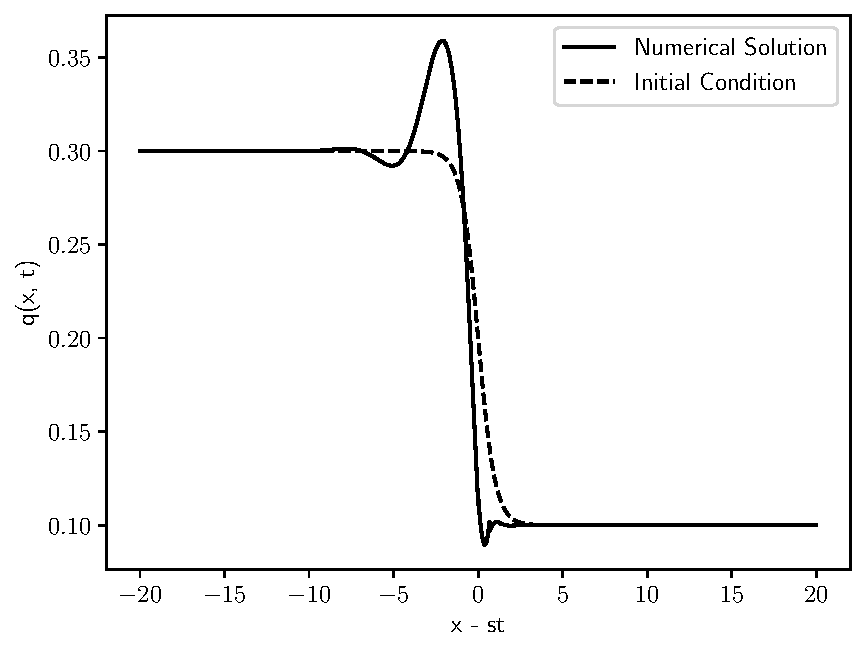
\includegraphics[scale=0.5]{figures/case_1_1.pdf}
  \caption{Case 1: Unique Lax Shock}\label{fig:case1}
\end{figure}

\subsubsection{Case 2: Multiple Lax Shocks}\label{sssec:case2}
If the left state is increased to \(q_l = 0.3323\), then the wave profile is no
longer unique.
In this case the steady traveling wave depends on the initial conditions.

For the following initial conditions,
\begin{equation}
  q_0(x) = \p{\tanh{-x} + 1} \frac{q_l - q_r}{2} + q_r\label{eq:case2_1}
\end{equation}
the behavior is the same as in case 1.
The numerical solution for this initial condition is shown in Figure~\ref{fig:case2}

Now consider the following initial conditions,
\begin{equation}
  q_0(x) =
  \begin{cases}
    \p{\p{0.6 - q_l}/2} \tanh{x} + \p{\p{0.6 + q_l}/2} & x < 5 \\
    -\p{\p{0.6 - q_r}/2} \tanh{x - 10} + \p{\p{0.6 + q_r}/2} & x > 5
  \end{cases}.\label{eq:case2_2}
\end{equation}
The reader might expect this initial condition to approach the traveling wave shown
earlier as it has the same far field boundary values, however this is not the case.
The traveling wave profile that is approaches is shown in Figure~\ref{fig:case2}.

\begin{figure}
  \centering
  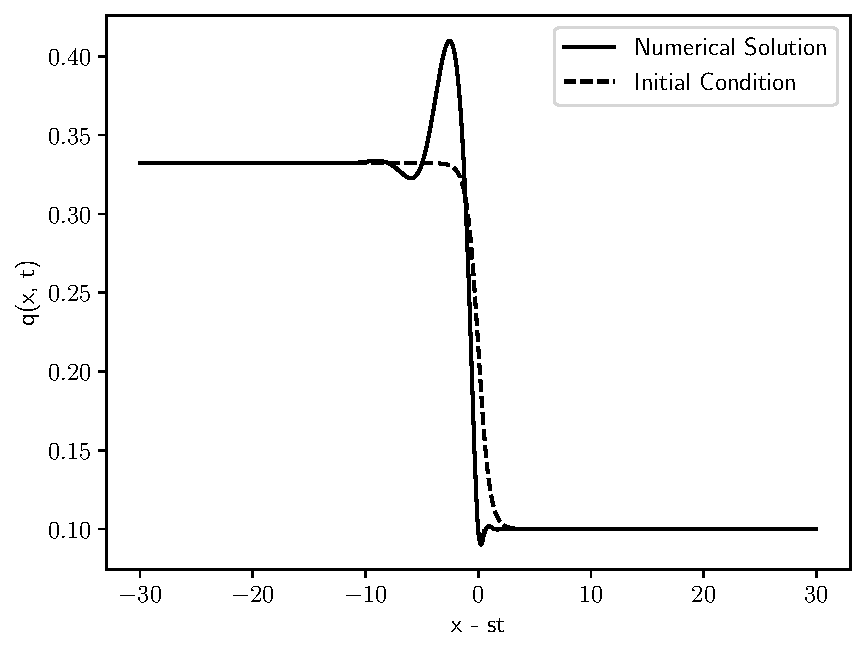
\includegraphics[scale=0.35]{figures/case_2_1.pdf}
  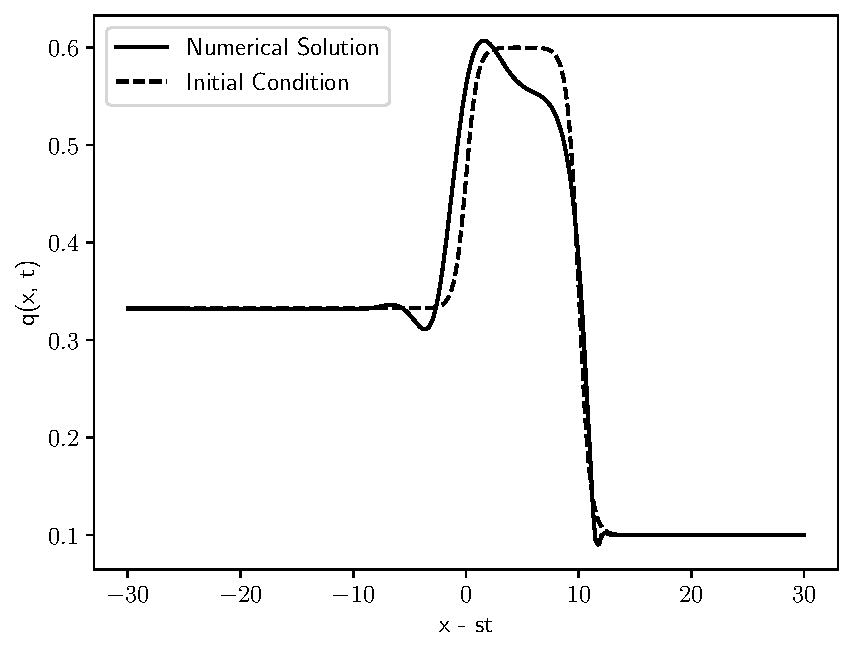
\includegraphics[scale=0.35]{figures/case_2_2.pdf}
  \caption{Case 2: Multiple Lax Shocks}\label{fig:case2}
\end{figure}

These are not the only possible wave profiles possible with these left and right
states.
Figure~\ref{fig:case2_3} shows the result for the following initial condition,
\begin{equation}
  q_0(x) =
  \begin{cases}
    \p{\p{0.6 - q_l}/2} \tanh{x} + \p{\p{0.6 + q_l}/2} & x < 10 \\
    -\p{\p{0.6 - q_r}/2} \tanh{x - 20} + \p{\p{0.6 + q_r}/2} & x > 10
  \end{cases}\label{eq:case2_3}.
\end{equation}
This initial condition has a larger hump then equation~\eqref{eq:case2_2}, and the
traveling wave reflects this aspect.
In this case the traveling wave is not a steady wave, and there are in fact
two shocks.
The right shock is an undercompressive shock and the left shock is a traditional
compressive shock.
Both shocks travel slower than the moving reference frame.
They also travel at different speeds from one another so the wave profile changes over
time.
\begin{figure}
  \centering
  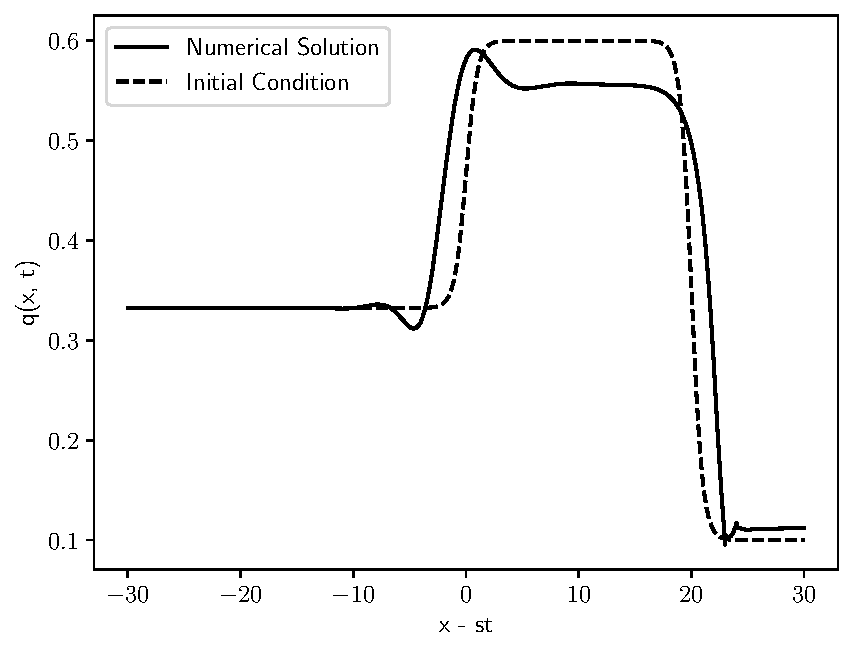
\includegraphics[scale=0.5]{figures/case_2_3.pdf}
  \caption{Case 2: Multiple Lax Shocks}\label{fig:case2_3}
\end{figure}

\subsubsection{Case 3: Undercompressive Double Shock}\label{sssec:case3}
For the left state in the next regime, there is again a unique shock profile for all
initial conditions.
However this shock profile is not the single Lax shock seen in Case 1.
With the following initial conditions,
\begin{equation}
  q_0(x) = \p{\tanh{-x} + 1} \frac{q_l - q_r}{2} + q_r
\end{equation}
where \(q_l = 0.4\) and \(q_r = 0.1\), figure~\ref{fig:case3} shows a double shock
structure.
Similar to figure~\ref{fig:case2_3}, we see a undercompressive shock on the right
and a Lax shock on the left.
\begin{figure}
  \centering
  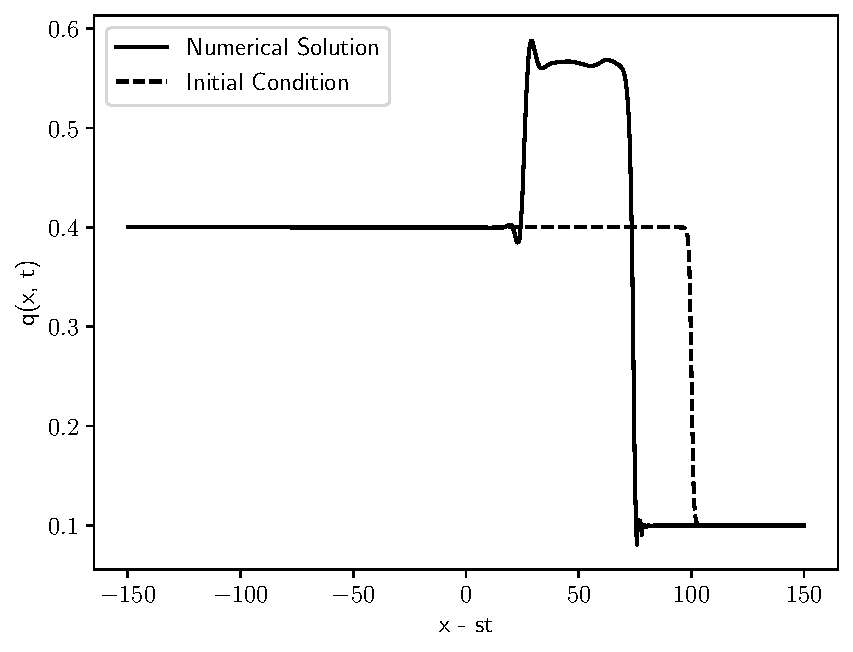
\includegraphics[scale=0.5]{figures/case_3_1.pdf}
  \caption{Case 3: Undercompressive Double Shock}\label{fig:case3}
\end{figure}

\subsubsection{Case 4: Rarefaction-Undercompressive Shock}\label{sssec:case4}
The final traveling wave structure appears when the left state is greater than the
undercompressive shock height.
In this case we see a rarefaction wave along with the undercompressive shock.
Figure~\ref{fig:case4} shows the numerical solution for initial condition
\begin{equation}
  q_0(x) = \p{\tanh{-x + 110} + 1} \frac{q_l - q_r}{2} + q_r
\end{equation}
where \(q_l = 0.8\) and \(q_r = 0.1\).
Note that the rarefaction wave and undercompressive shock are traveling at different
speeds so they seperate from each other.
\begin{figure}
  \centering
  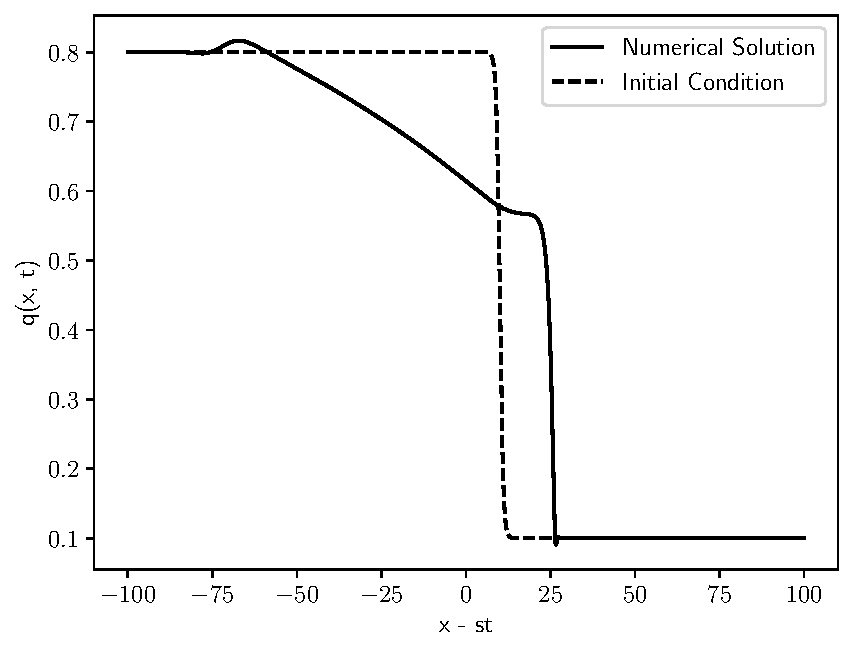
\includegraphics[scale=0.5]{figures/case_4_1.pdf}
  \caption{Case 4: Rarefaction-undercompressive shock}\label{fig:case4}
\end{figure}

% \bibliographystyle{plain}
% % \vspace{-20pt}
% \begingroup
%     \setlength{\bibsep}{13.2pt}
%     \linespread{1}\selectfont
%     \bibliography{refs}
% \endgroup
\clearpage
\pagebreak
% \chapter{PAPER 4 TITLE GOES HERE}
% \label{polymer_fibers1}

\begin{center}
    A paper accepted by \textit{Name of the Journal} \\
    First Author and Second Author
\end{center}

\section{Abstract}
This is the text of my abstract that is part of the thesis itself.
The abstract describes the work in the first paper general. You can use the same abstract as your paper here.

%\pagebreak %remove if needed

% Please include sections as the paper has, some of the following sections are meant as examples of what can be done, the bibliography should be made as given
%\section{Overview}

This is the opening paragraph to my thesis which
explains in general terms the concepts and hypothesis
which will be used in my thesis.

With more general information given here than really
necessary.

\section{Introduction}

Here initial concepts and conditions are explained and
several hypothesis are mentioned in brief.

Of course, data on this as seen in Table~\ref{data}
is few and far between.

\begin{table}[h!tb] \centering
\isucaption{Moon Data}
\label{data}
% Use: \begin{tabular{|lcc|} to put table in a box
\begin{tabular}{lcc} \hline
\textbf{Element} & \textbf{Control} & \textbf{Experimental} \\ \hline
Moon Rings & 1.23 & 3.38 \\
Moon Tides & 2.26 & 3.12 \\
Moon Walk & 3.33 & 9.29 \\ \hline
\end{tabular}
\end{table}


\subsection{Hypothesis}

Here one particular hypothesis is explained in depth
and is examined in the light of current literature.

Or graphically as seen in Figure~\ref{mgraph}
it is certain that my hypothesis is true.

\begin{figure}[h!tb] \centering

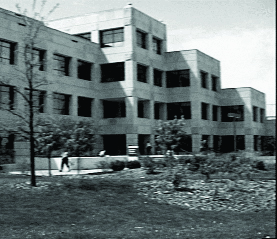
\includegraphics{Images/dc5}

\isucaption{Durham Centre}
\label{mgraph}
\end{figure}

\subsubsection{Parts of the hypothesis}

Here one particular part of the hypothesis that is
currently being explained is examined and particular
elements of that part are given careful scrutiny.

% Below \subsubsection
% Sectional commands: \paragraph and \subparagraph may also be used

\subsection{Second Hypothesis}

Here one particular hypothesis is explained in depth
and is examined in the light of current literature.

\subsubsection{Parts of the second hypothesis}

Here one particular part of the hypothesis that is
currently being explained is examined and particular
elements of that part are given careful scrutiny.

\section{Criteria Review}

Here certain criteria are explained thus eventually
leading to a foregone conclusion.

\section{Results}

\section{Conclusion}\label{conclusion3}

The conclusion of the paper goes here.

% This section may or may not be included
\section{Appendix: supplemental procedure description}
If there is an appendix that needs to go with the paper it can be as a section

\subsection{Procedure details}
Details of the paper specific appendix procedures

%\cite{allen}, \cite{bruner}
\cite{Rad87}
\cite{MOR91}, \cite{Lom73}
\cite{Lom91}, \cite{Lom92}
\cite{dB59}

% \section{Bibliography}
% \bibliographystyle{plain}
% % \vspace{-20pt}
% \begingroup
%     \setlength{\bibsep}{13.2pt}
%     \linespread{1}\selectfont
%     \bibliography{master_bib}
% \endgroup
\clearpage
\pagebreak
\chapter{Conclusion}
\label{conclusion}
This thesis has shown a discontinuous Galerkin method for solving a Thin-Film equation.

The implicit-explicit time-stepping allows for reasonable time steps to be taken given
the stiffness of the problem.
The nonlinear problem was able to be solved without a Newton iteration.
In fact a Picard Iteration was used, and it was demonstrated that only a minimal
number of iterations were required to achieve high accuracy.
We have demonstrated up to third order accuracy, and this was achieved with the number
of Picard iterations less than or equal to the order of accuracy.

\clearpage
\pagebreak


%%%%%% bibliographies

%\clearpage
%% \nocite{*}
\unappendixtitle
\newpage
\phantomsection
\addcontentsline{toc}{chapter}{BIBLIOGRAPHY}
\section*{BIBLIOGRAPHY}
\bibliographystyle{plain}
\vspace{-20pt}
\begingroup
   \setlength{\bibsep}{14.5pt}
   \linespread{1}\selectfont
   \bibliography{refs}
\endgroup

% Renders the citations but does not show the bibliography at the end of the thesis
% \newsavebox\mytempbib
% \savebox\mytempbib{\parbox{\textwidth}{\bibliography{master_bib}}}

\clearpage
\pagebreak
% % Appendix1 file from standard thesis template

\appendixtitle 
\appendix


%% Use the following two lines for single appendix
%\unappendixtitle
%\singleappendixtitle

\chapter{ADDITIONAL MATERIAL} 
This is now the same as any other chapter except that
all sectioning levels below the chapter level must begin
with the *-form of a sectioning command.

\section*{More stuff}

Supplemental material.

 % Instruction for single appendix look below
% % An example second appendix from the example thesis thesis.tex.
\chapter{STATISTICAL RESULTS}

This is now the same as any other chapter except that
all sectioning levels below the chapter level must begin
with the *-form of a sectioning command.

\section*{Supplemental Statistics}

More stuff.

\end{document}
